\documentclass[tikz,border=6pt]{standalone}
\usepackage{tikz}
\usetikzlibrary{arrows.meta,automata,positioning}
\begin{document}
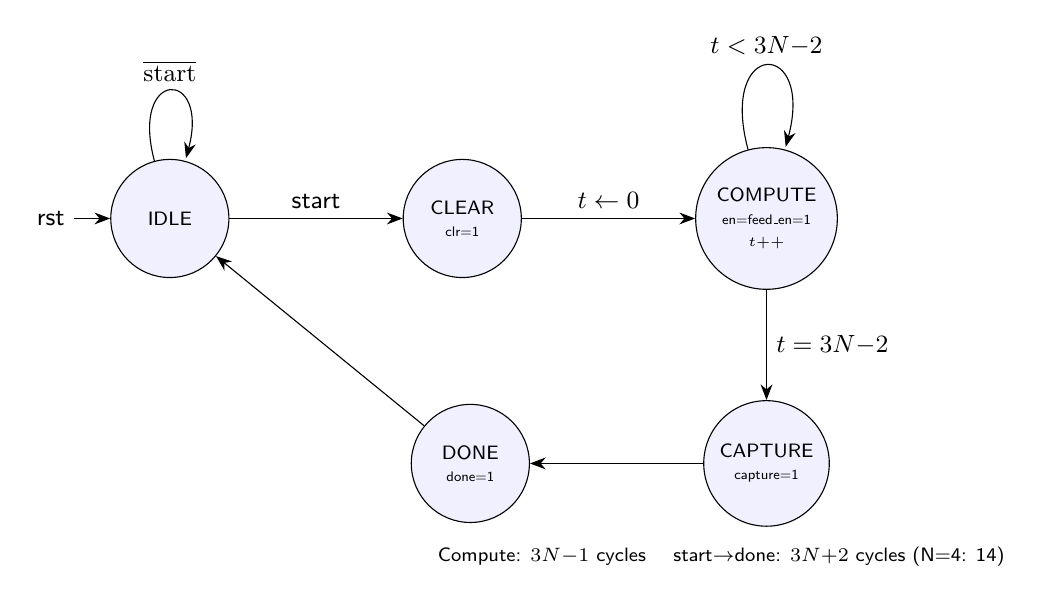
\begin{tikzpicture}[font=\sffamily\small, >={Stealth[length=2mm]}, node distance=14mm and 22mm,
  every state/.style={draw, fill=blue!6, minimum size=15mm, align=center, font=\sffamily\scriptsize}]
\node[state, initial, initial text={rst}] (idle) {IDLE};
\node[state, right=of idle] (clr) {CLEAR\\\tiny clr=1};
\node[state, right=of clr] (cmp) {COMPUTE\\\tiny en=feed\_en=1\\\tiny $t{+}{+}$};
\node[state, below=of cmp] (cap) {CAPTURE\\\tiny capture=1};
\node[state, left=of cap] (done) {DONE\\\tiny done=1};
\draw[->] (idle) edge node[above]{start} (clr)
          (clr) edge node[above]{$t\leftarrow0$} (cmp)
          (cmp) edge[loop above] node{$t<3N{-}2$} (cmp)
          (cmp) edge node[right]{$t=3N{-}2$} (cap)
          (cap) edge (done)
          (done) edge node[below left]{} (idle)
          (idle) edge[loop above] node{$\overline{\mathrm{start}}$} (idle);
\node[font=\sffamily\scriptsize, align=left, below=4mm of done.south west, anchor=north west]
  {Compute: $3N{-}1$ cycles \quad start$\to$done: $3N{+}2$ cycles (N=4: 14)};
\end{tikzpicture}
\end{document}
